\section{Problema 1: Plan de vuelo}

\subsection{Presentación del problema}

Se quiere crear un sitio web para reservas de pasajes de avi\'on. El sitio debe tener un sistema de b\'usqueda de itinerarios de vuelo. Un itinerario de vuelo, es una sucesi\'on de vuelos los cuales logran llevar a un pasajero hacia un destino. Dado una ciudad de salida, y una ciudad de llegada, se busca crear un itinirario de vuelos que vaya desde la ciudad de salida hasta la de llegada.

Dentro de este itinerario, cada vuelo tiene un horario de despegue y uno de aterrizaje. 

Para poder ser un itinerario v\'alido, la ciudad de destino de un vuelo dentro del itinerario, tiene que ser la ciudad de llegada del pr\'oximo o directamente el destino final donde queriamos llegar, y en particular cada vez que llego a una ciudad debo esperar al menos dos horas desde el aterrizaje, para poder tomarme cualquier vuelo que salga desde esa ciudad, lo cual resulta l\'ogico dado que una persona puede necesitar al menos ese tiempo para tr\'amites de aeropuerto.

Es por eso que se nos pide el mejor itinerario, teniendo al menos dos horas entre cada vuelo, donde mejor itinerario es el que primero aterriza en la ciudad destino final.

Adem\'as se nos pide que la resoluci\'on de este problema se implemente en un complejidad no peor a O($N^{2}$) donde N es la cantidad de vuelos totales que existen en todo el sistema (formen parte del itinerario o no).

\newpage
\subsubsection{Formalmente}


Sea Ciudad un renombre de String.

Sea Vuelo una tupla $<$despegue:Nat, aterrizaje:Nat, origen:Ciudad, destino:Ciudad$>$

Dado $vuelos$:Conj(Vuelo):

Llamemos a $ciudadades$:Conj(Ciudad) al conjunto tal que:
\begin{align*}
(\forall c:Ciudad, c \in ciudades)  \Leftrightarrow (\exists v:Vuelo)/ v \in vuelos \wedge (v.origen \equiv c \vee v.destino \equiv c))
\end{align*}
Dadas $a,b$:Ciudad, $a,b \in ciudades$. 

Sean los enunciados:


\begin{align*}
esItinerarioValido(S:Sec<Vuelo> , a:Ciudad, b:Ciudad) \equiv \\
(S_{0}.origen \equiv a \wedge S_{S.tamanio-1}.destino \equiv b) \wedge \\ 
(\forall i:Nat, 0 \leq i <S.tamanio-1)(S_{i}.destino \equiv S_{i+1}.origen 
\wedge S_{i}.aterrizaje + 2 \leq S_{i+1}.despegue))
\end{align*}

Este enunciado indica si una secuencia de vuelos en particular, no vacia, es un itinerario v\'alido para nuestro problema.

\begin{align*}
Sec<Vuelo> s \subseteq Conj(Vuelo) c \equiv 
(\forall i:Nat, 0 \leq i \geq s )(s_{i} \in  c)
\end{align*}
 
Este enunciado es un abuso de notaci\'on para indicar que una secuencia de vuelos esta contenidad en un conjunto de vuelos.


Se nos pide encontrar $S$:Sec$<$Vuelo$>$ tal que 
\begin{align*}
esItinerarioValido(S,a,b) \wedge (S \subseteq vuelos) \wedge \\
(\forall S':Sec<Vuelo> / (esItinerarioValido(S',a,b)) \wedge (S' \subseteq vuelos) \implies \\  
S_{S.tamanio-1}.aterrizaje) \leq S'_{S'.tamanio-1}.aterrizaje))
\end{align*}

\newpage
\subsection{Resolución}

Habiendo caracterizado la soluci\'on a nuestro problema en lenguaje formal, vamos a tratar de encontrar una implementaci\'on para un algoritmo que devuelva una instancia de esa soluci\'on.

Dados C:Conj(Vuelo), $inicio$:Ciudad, $destino$:Ciudad y el instante T:Nat, que va a ser un instante de tiempo.

Sea la funci\'on:
\begin{align*}
boolean\;ExisteVuelo(Conj(Vuelo) \; vuelos,\; Ciudad\;inicio,\;Ciudad\;destino,\;Nat \;T) \equiv\\
(inicio == destino) \vee (\exists v:Vuelo, v \in vuelos) / (v.inicio == inicio \; \wedge \\ 
v.despegue - 2 \geq T) \\
\wedge ExisteVuelo(vuelos,v.destino, destino, v.aterrizaje)))  
\end{align*}

Esta expresi\'on nos indica si dado un instante T, en alguna ciudad c existe una secuencia de vuelos v\'alida que nos lleva desde c hasta la ciudad destino que queremos llegar.

Solo nos va a interesar un vuelo v tal que exista un itinerario v\'alido hasta tomarnos v y que exista un itinerario v\'alido hasta nuestra ciudad destino a partir de tomarnos v, esta noci\'on va a definir nuestro conjunto de vuelos v\'alidos.

Como se puede notar el enunciado de ExisteVuelo, esta definido recursivamente.

Dados C:Conj(Vuelo), $inicio$:Ciudad, $destino$:Ciudad.

Podemos definir el conjunto Validos(C,inicio,destino):Conj(Vuelo), como:
\begin{align*}
(\forall v:Vuelo, v \in Validos(C,inicio,destino)) \Leftrightarrow ((v.origen == inicio \;\vee \\
(\exists v':Vuelo, v' \in Validos(C,inicio,destino) / v'.destino == v.origen \wedge v'.aterrizaje + 2 \leq\\ v.despegue)) \wedge ExisteVuelo(C,v.destino,destino,v.aterrizaje) \wedge v \in C)
\end{align*}

Dado este conjunto podemos definir el VueloMinimo:Vuelo, tal que VueloMinimo pertenezca al conjunto de vuelos v\'alidos y VueloMinimo sea el primero que aterrice en cada ciudad..

Dados C:Conj(Vuelo), $inicio$:Ciudad, $destino$:Ciudad, $ciudad$:Ciudad.
\begin{align*}
VueloMinimo(C,inicio,destino,ciudad) \equiv v:Vuelo \Leftrightarrow (v \in Validos(C,inicio,destino) \wedge\\ v.destino == ciudad \wedge (\forall v':Vuelo, v' \in Validos(C,inicio,destino) \wedge \\
v'.destino == ciudad) \implies v.aterrizaje \leq v'.aterrizaje)
\end{align*}

Nuestro algoritmo va a obtener este VueloMinimo $v$ para cada ciudad, tal que $v$ pertenezca al conjunto de vuelos v\'alidos desde inicio hasta destino . Las caracteristica de VueloMinimo es que es el primero de los vuelos que llegan a una ciudad por un itinerario v\'alido desde inicio hasta destino.

En particular se puede observar que, cualquier itinerario v\'alido que contenga al vuelo m\'inimo de la ciudad destino, es decir a VueloMinimo(C,inicio,destino,destino) en su \'ultimo vuelo va a ser soluci\'on de nuestro problema. 

Esto es ya que no va existir un itinerario v\'alido que aterrice antes en destino, que cualquier itinerario v\'alido que contenga a ese vuelo.

Luego la soluci\'on s:Sec$<$Vuelo$>$ que se devuelve como itinerario de vuelos por nuestro algoritmo, cumple:

\begin{align*}
esItinerarioValido(s,inicio,destino) \wedge s \subseteq C \wedge \\
(\forall v:Vuelo, v \in s)(s == VueloMinimo(C,inicio,destino,s.destino))
\end{align*}

\newpage
\subsection{PseudoC\'odigo a la c++}


Nuestro algoritmo final quedaria de la siguiente manera:

Definimos Color como un enum $[$BLANCO,ROJO,VERDE$]$

Definimos un Aeropuerto como un tupla 

\begin{align*}
\langle ciudad:Ciudad,vuelosQueSalen:
Conj(Vuelo),vuelosQueLlegan:Conj(Vuelo),\\
id:Nat,primerVueloQueSaleYLlega:Vuelo,ultimoVueloQuellega:Nat \rangle 
\end{align*}

\begin{algorithm}[H]
\begin{algorithmic}[1]
\STATE Aeropuerto[] aeropuertos = construirArrayDeAeropuertos(vuelos,inicio,final)
\STATE Sec$\langle$Vuelo$\rangle$ $itinerario$ $=$ $[]$

$/*$ Esta sesgada la funcion con T $=$ -2 ya que vamos a preguntar si existeVuelo a partir de T $=$ 0.
En la posicion 0 se encuentra el aeropuerto de la ciudad inicial, y en la posici\'on 1, el de la ciudad final $*/$
\IF{(existeVuelo(aeropuertos, aeropuertos[0],aeropuertos[1],-2))}
	\STATE Vuelo min = aeropuerto$[1]$.primerVueloQueSaleYLlega
\STATE $itinerario$.agregar(min,0)
\WHILE {(min.inicio != inicio) }
	\STATE Vuelo min $=$ vueloMinimo.primerVueloQueSaleYLlega
	\STATE $itinerario$.agregar(min,0)
\ENDWHILE
\ENDIF
\RETURN $itinerario$
\caption{Sec$\langle$Vuelo$\rangle$ itinerario(Conj(Vuelo) vuelos, Ciudad inicio, Ciudad final)}% $\rightarrow$ int proximo}
\end{algorithmic}
\end{algorithm}

\newpage
La siguiente funci\'on obtiene el conjunto de vuelos v\'alidos desde una ciudad inicio hasta una ciudad destino, en el instante T, si el conjunto existe devuelve TRUE, sino FALSE.

\begin{algorithm}[H]
\begin{algorithmic}[1]
\IF {(inicio $==$ destino)}	
		\RETURN TRUE
\ENDIF
\IF {(t + 2 $\leq$ inicio.ultimoVueloQueLlega())}	
		\RETURN TRUE
\ENDIF
\STATE boolean llego $=$ false;
\STATE Conj(vuelo) vuelos $=$ inicio$.$vuelosQueSalen;
\STATE inicio$.$vuelosQueSalen $=$ $\emptyset$;
\STATE Conj(vuelo) vuelosNoAnalizados $=$ $\emptyset$;
\FOR{(Vuelo v $:$ vuelos)}	    
    \IF {(v.despegue $\geq$ t+2)}	
        \IF{(v.color $==$ BLANCO)}     				        	
        		\IF {(existeVuelo(aeropuertos,v.destino,final,v.aterrizaje)}
				\STATE llego = true
				\STATE v.color = VERDE
				\IF {(inicio.ultimoVueloQuellega $<$ v.llegada)}	
					\STATE inicio.ultimoVueloQuellega = v.llegada
				\ENDIF
				\IF {(vuelo.destino.primerVueloQueSaleYLlega.llegada $>$ v.llegada)}	
					\STATE vuelo.destino.primerVueloQueSaleYLlega = v
				\ENDIF

			\ELSE
				\STATE v.color = ROJO								
	    		\ENDIF    			
		\ENDIF
	\ELSE
		\STATE vuelosNoAnalizados.agregar(v)										    
    \ENDIF
\ENDFOR
\STATE inicio$.$vuelosQueSalen $=$ vuelosNoAnalizados;
\RETURN $llego$
\caption{boolean existeVuelo(Aeropuerto[] aeropuertos, Aeropuerto inicio, Aeropuerto final, int t)}% $\rightarrow$ int proximo}
\end{algorithmic}
\end{algorithm}

Esta funci\'on se llama recursivamente con los vuelos de la ciudad inicio. El caso base de la funci\'on es cuando llega a la ciudad destino o cuando llega a un camino de vuelos v\'alidos que se pueda tomar desde el instante T, entonces devuelve true.

Si itera por todos los vuelos de ciudad inicio, y si ning\'un vuelo llega a destino ni sus llamadas recursivas respectivas, entonces devuelve false.

Cada vez que detecte que un vuelo $v$ llega al destino o a un camino de vuelos que me lleven a destino, colorea de verde a $v$ y actualiza dos datos:

Un puntero en v.destino, al primer vuelo que aterriza en $v$.destino y llega al destino.

Un Nat que representa el instante de aterrizaje del \'ultimo vuelo que aterriza en Inicio, y llega a destino.

Luego el conjunto de vuelos que estan contenidos en alg\'un itinerario v\'alido son los que marco de verde.

La funci\'on es recursiva, para poder cumplir la complejidad requerida, creamos un puntero a la lista de vuelos de un aeropuerto, y en caso de tener que hacer una llamada recursiva, se apunta a null esa lista, para que dado que entro en una recursion de un vuelo, no volver a consultar por los mismos vuelos de una ciudad. Esto se basa en el principio de que si dentro de una recursi\'on visito la misma ciudad, el T de la primera recursi\'on va a ser menor al de la segunda, por lo tanto los vuelos que me pueda tomar en la segunda, ya voy a poder evaluarlos en la primera.

Si existe un vuelo que llega a la misma ciudad desde una recursi\'on, se genera un ciclo.

Ese vuelo en particular no nos interesa, ya que cualquier camino de vuelos que pueda existir a partir del instante de llegada de ese vuelo a la ciudad C, tambien lo voy a poder hacer con el instante de llegada de la primera recursion a C, ya que es estrictamente menor por lo tanto todos los vuelos que est\'en disponibles en la segunda iteraci\'on tambi\'en van estarlo en la primera. 

Por lo tanto dado que se entra en una recursi\'on desde una ciudad inicio, se vacian los vuelos que salen de esa ciudad, para no volver a iterarlos dentro de la recursi\'on y no generar este ciclo.

\newpage

La siguiente funcion construye un array de aeropuertos, en complejidad O(N.Log(N))

\begin{algorithm}[H]
\begin{algorithmic}[1]
\STATE Conj(Ciudad) ciudades = null
\STATE ciudades.agregar(inicio)
\STATE ciudades.agregar(final)
\FOR {(Vuelo vuelo: Vuelos)}	
	\STATE ciudades.agregar(vuelo.origen)
	\STATE ciudades.agregar(vuelo.destino)
\ENDFOR
\STATE Aeropuerto[] aeropuertos = new Aeropuerto[ciudades.size];
\STATE Mapa$\langle$Ciudad, Nat$\rangle$ ids $=$ $\emptyset$
\STATE ids.agregar(inicio,0)
\STATE ids.agregar(final,1)
\STATE aeropuertos[0] = new Aeropuerto (inicio,$\emptyset$,$\emptyset$,0)
\STATE aeropuertos[1] = new Aeropuerto (final,$\emptyset$,$\emptyset$,1)
\STATE ciudades.remover(inicio)
\STATE ciudades.remover(final)
\STATE Nat i = 2
\FOR {(Ciudad ciudad: ciudades)}	
	\STATE aeropuertos[i] = new Aeropuerto (ciudad,$\emptyset$,$\emptyset$,i)
	\STATE ids.agregar(ciudad,i++)
\ENDFOR
\STATE i $=$ 1
\FOR {(Vuelo vuelo: Vuelos)}	
	\STATE vuelo.id = i++	
	\STATE vuelo.color = BLANCO	
	\STATE int id = ids.obtener(vuelo.origen)
	\STATE aeropuertos[id].vuelosQueSalen().agregar(vuelo)
	\STATE id = ids.obtener(vuelo.destino)
	\STATE aeropuertos[id].vuelosQueLlegan().agregar(vuelo)
\ENDFOR
\RETURN ciudades
\caption{Aeropuerto[] construirArrayDeAeropuertos(Conj(Vuelo) vuelos, Ciudad inicio, Ciudad final)}% $\rightarrow$ int proximo}
\end{algorithmic}
\end{algorithm}
Esta funcion va a asignarle un id a cada una de las ciudades y luego construir un array donde en la posicion i, se encuentra la ciudad con id $=$ 1.

Implementada sobre un trie o sobre un hashmap, para el diccionario de ids me daria una complejidad al algoritmo de crear el mapa de aeropuertos cercana a O(n) en n numero de vuelos. Los nombres de la ciudad tienden a ser Strings de bajo costo de procesamiento en un trie, y en un hashmap la cantidad total de ciudades con aeropuertos en el mundo, es un numero relativamente bajo, por lo tanto se podr\'ia implementar de forma eficiente.
Nuestra implementaci\'on usa un treeset, asi que la complejidad de crear nuestros aeropuertos es O(n.log(n))



\newpage

\subsection{Demostración}
Para obtener el conjunto de vuelos v\'alidos vamos a implementar una funci\'on recursiva que itere por los vuelos que salen desde la ciudad inicial hasta la ciudad final, los siguientes enunciados son importantes para entender en que se basa el algoritmo.

Dados, $vuelos$:conj(Vuelo), una ciudad $C$, $inicio$:Ciudad y $destino$:Ciudad

Corolario 1:

\begin{align*}
(ExisteVuelo(vuelos,inicio, C, 0) \wedge (\exists v:Vuelo, v \in Validos(vuelos,inicio,C))\\
(v.destino == C \wedge ExisteVuelo(vuelos,C, destino, v.aterrizaje))) \implies \\ ExisteVuelo(vuelos,inicio, destino, 0)
\end{align*}
Corolario 2:

\begin{align*}
(\forall C':Ciudad / \exists v:Vuelo, v.inicio == C' \wedge v.destino == C)\\
(ExisteVuelo(vuelos,C,destino,v.aterrizaje) \implies \\
ExisteVuelo(vuelos,C',destino,v.despegue) \wedge v \in Validos(vuelos,C',destino)
\end{align*}
\begin{align*}
\end{align*}


Corolario 3:

Sea v:Vuelo tal que:
\begin{align*}
v.destino == C \wedge v \in Validos(vuelos,C,destino) \wedge\\
(\forall v':Vuelo, v' \in Validos(vuelos,C,destino)(v.aterrizaje \geq v'.aterrizaje))\\
\end{align*}
Entonces:
\begin{align*}
(\forall C':Ciudad / \exists w:Vuelo, w.inicio == C' \wedge w.destino == C)\\
w.aterizaje + 2 \leq v.despegue \implies w \in Validos(vuelos,C',destino) 
\end{align*}


\newpage

\subsection{Análisis de complejidad}
Nuestra implementaci\'on consta de tres partes:

1. Construir el array de aeropuertos.

2. Encontrar el conjunto de vuelos v\'alidos desde la ciudad origen hasta la ciudad destino.

3. Obtener un secuencia valida de Vuelos m\'inimos.

1.

Para construir el array de aeropuertos, lo que se hace es contar la cantidad de ciudades para crear un array de ese tamaño.
Para ello, se carga cada ciudad en un TreeSet. Como la cantidad de ciudades la podemos acotar por la cantidad de vuelos, ya que a lo sumo tenemos 2 ciudades por vuelo, sea N la cantidad de vuelos, la cantidad de ciudades maximas es de 2.N, por lo tanto el costo de crear este Set es a lo sumo O(N.Log(N))

Crear el array tiene una complejidad temporal de O(N) a lo sumo y espacial de 2.N.

Luego se le asocia un id a estas ciudades, que va a ser la posicion donde se van a encontrar en el array. Para poder asociarle este id se construye un mapa $\langle Ciudad,ID \rangle$.
Buscar en este mapa nos va a costar O(Log(N)) y construirlo O(N.Log(N)).

Luego se asocio cada vuelo a la posicion donde se encuentran la ciudad destino e inicio de ese vuelo.
Para ello se busca el id en el mapa. Entonces para asociar todos los vuelos tenemos la complejidad es de O(N.Log(N)).

Luego la complejidad final de construir el array es O(N.Log(N)).

2.

Sea i una llamada recursiva del algoritmo.

Sea $Inicio_{i}$:Ciudad, la ciudad inicial de la recursion i.

%Sea $T_{i}$:Nat, el instante T de la recursion i.


Antes de empezar a iterar por los vuelos que salen de $Inicio_{i}$, se borra el puntero a este conjunto en $Inicio_{i}$.

Si vuelvo a $Inicio_{i}$ en una instancia de recursion a partir de i,puedo asegurar que los vuelos que salen de $Inicio_{i}$, no van a estar incluidos.

Es decir, no existen ciclos en la recursi\'on, donde un ciclo seria volver a iterar por un vuelo que se haya iterado anterioremente.

Entonces para cualquier recursi\'on, se chequean a lo sumo todos los vuelos de cada ciudad.

Todos los vuelos de cada ciudad son exactamente N vuelos.

Cuando se genera una llamada recursiva se colorea el vuelo, por lo tanto ese vuelo nunca mas va a ser llamado recursivamente ya que se conoce el estado para cualquer instante de tiempo.

Entonces el algoritmo puedo tener tantas llamadas recursivas como vuelos distintos tenga.

El numero de vuelos distintos es N.

Y para cada llamada recursiva a lo sumo se itera exactamente una vez por cada vuelo.

Por lo tanto la cantidad total de vuelos que se iteran dado que se llego a una ciudad, en un instante T esta acotado por la cantida total de llamadas recursivas y la cantidad de vuelos que a lo sumo se iteran en cada una.

Existen a lo sumo N recursiones ya que existen a lo sumo N vuelos que puedo llamar recursivamente, y una recursion tiene un complejidad a lo sumo de O(N) para conocer su estado.

Luego la cantidad de iteraciones m\'axima que se realizan tiene una complejidad a lo sumo O($N^{2})$.

3.

Para construir nuestra secuencia de vuelos soluci\'on vamos a iterar por los vuelos m\'inimos de cada ciudad que llegan a destino.
Un vuelo minimo para una ciudad C, es de todos los vuelos que llegan a C y pertenecen a un itinerario v\'alido desde inicio hasta la ciudad final, el primero que aterriza en C. 

%Todos los vuelos que salen de C y pertenecen a un itinerario v\'alido, pueden ser tomados por un pasajero, a partir de aterrizar en C, con al menos un vuelo que aterrice en C y pertenezca a un itinerario valido.

%El vuelo m\'inimo es el que primero aterriza y pertenece a un itinerario valido, por lo tanto cualquier vuelo que salga de C y pertenezca a un itinerario valido, puedo ser tomado a partir de aterrizar en C con el vuelo minimo.

Suponemos que no existe vuelos que ciclan a la misma ciudad, es decir que su destino y origen es el mismo. (informalmente podemos descartar estos vuelos porque si existe una solucion para ellos, existe una solucion para otro vuelo pero que no genere un ciclo).

Sea s un secuencia de vuelos, tal que s es un itinerario v\'alido de vuelos minimos.

\begin{align*}
(\forall i,j:Nat, i,j<S.tamanio \wedge i<j)(S_{i}.aterrizaje < S_{j}.despegue
\vee S_{i}.destino == final)
\end{align*}

Luego si S contiene un ciclo, va a existir al menos un vuelo, que pertenezca a ese ciclo,(en particular va a ser el vuelo que cierre ese ciclo), no va a cumplir este invariante, ya que el aterrizaje de un vuelo es siempre mayor a su despegue (en particular por como lo definimos podr\'ia existir m\'as de un vuelo m\'inimo por ciudad, pero igual fallar\'ia ya que el horario de aterrizaje deber\'ia ser igual para todo vuelo m\'inimo de una ciudad).

Por lo tanto un itinerario v\'alido de vuelos m\'inimos no tiene ciclos. 

El itinerario v\'alido mas largo que puede existir sin ciclos es a lo sumo de tamaño N.

Por lo tanto obtener el itinerario cuesta a lo sumo O(N).


Luego la complejidad total del algoritmo es O(N.Log(N)) + O($N^{2})$ + O(N) $=$ O($N^{2})$
\subsection{Tests de complejidad}

Para analizar y testear tanto complejidad como correctitud del algoritmo implementado para la resoluci\'on del problema  realizamos los siguientes testeos:

\begin{itemize}
  \item Test de casos borde.
  \item Test de generaci\'on de casos pseudo aleatorios.
  \item Test de analisis de peor caso.
\end{itemize}

\newpage

\subsubsection{Test de casos borde}


Los siguientes test fueron implementados:

\begin{itemize}
  \item testUnVuelo() $=$ Chequea dado un conjunto de vuelos, tal que todos los vuelos salen de inicio, que la soluci\'on sea el de menor aterrizaje.
  \item 	testSinVuelos() $=$ Dado un conjunto vacio de vuelos, asegura la soluci\'on es "no".
  \item test2HorasDeDiferenecia() Asegura que la soluci\'on contenga 2hs de diferencia entre vuelo y vuelo.
  \item testCiclosALaMismaCiudad() $=$ Asegura dado que existe un ciclo a la misma ciudad, el algoritmo devuelva una soluci\'on v\'alida.
  \item testLlegoPorUnCaminoAntesQueDerecho() $=$ Asegura que la soluci\'on sea el camino que m\'as temprano llegue y no el m\'s corto.
  \item testCiclos $=$ Asegura dado que existen ciclos en mi conjunto de vuelos (es decir vuelvo a la misma ciudad desde un vuelo) el algoritmo retorne una soluci\'on v\'alida.
\end{itemize}

\subsubsection{Test de generaci\'on de casos pseudo aleatorios}

Se genero instancias pseudo-aleatorias de entrada para el algoritmo.

La pseudo-aleatoridad se basaba en generar N vuelos aleatorios, es decir vuelos donde el punto de partida y el de aterrizaje sean un elemento random, distintos dentro de un conjunto acotada de ciudades.

Tomamos la cota para la cantidad de ciudades como N/20. Esta cota se da para obtener instancias relativamente reales, y no es las cuales haya muchos vuelos que el algoritmo nunca recorra (estos casos deber\'ian tener un tiempo relativamente menor para obtener una soluci\'on).


Se tomo el tiempo de corrida para la misma instancia k veces, y de esas corridas se elegio el de menor tiempo de respuesta.

Luego para cada N distinto se obtuvo este gr\'afico.

TODO

Como se puede apreciar, la tendencia bajo esta pseudo-aleatoridad tambi\'es es polinomial en el tamaño de entrada.

\newpage
\subsubsection{Test de analisis de peor caso}

Una instancia donde encontramos que la complejidad iba a tender a nuestra cota de O($N^{2}$), es cuando la ciudad inicial tiene N/2 vuelos, que aterrizan en C:Ciudad, y luego C tiene N/2 vuelos que van desde C hasta cualquier otra ciudad con un horario de despegue menor a cualquier vuelo desde la ciudad inicial.

Como el algoritmo no puede saber en cada recursi\'on si va a existir un vuelo v\'alido para el T de entrada, tiene que iterar por todos los vuelos de C. Como desde inicio salen N/2 vuelos, la complejidad la funci\'on existeVuelo es $N^{2}$/4

Creemos que toda instancia de problema, deber\'ia estar sobre esta cota, ya que si existiesen mas ciudades alcanzables desde inicio, dividiria en partes mas pequeñas la iteraci\'on de vuelos de cada ciudad.

Si existiesen mas ciudades alcanzables desde inicio hasta C, los vuelos que lleguen a esas ciudades estar\'ian coloreados luego de alguna una llamada recursiva, por lo tanto tampoco se iterarian de nuevo.

Para el gr\'afico siguiente se generaron entradas diferentes de N y para cada entrada se corri\'o el algoritmo un numero K de veces.

Para cada entrada de tamaño S, se tomo el tiempo de corrida de esa entrada, y de todas las instancias de igual tamaño se considero el menor tiempo en el que el algoritmo devolv\'ia una soluci\'on.

Como se corri\'o dentro de una m\'aquina deterministica, este es el mejor tiempo que se pudo obtener para cada instancia. 

Luego obtuvimos se obtuvo el siguiente gr\'afico:

\begin{figure}[ht]
	\begin{minipage}[t]{\linewidth}
		\centering
		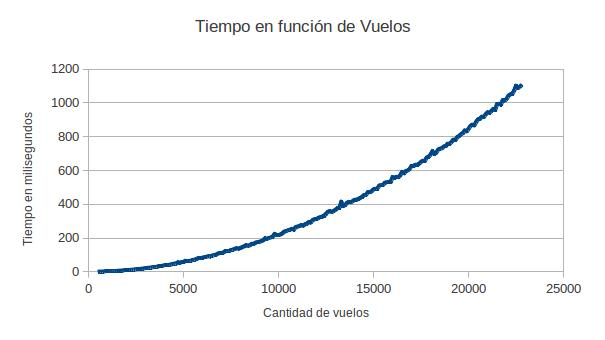
\includegraphics[width=\textwidth]{GraficoDeVuelosYTiempo.jpg}
	\end{minipage}	
\end{figure}

\subsubsection{Comparaci\'on}

Luego se corrio y grafico la salida, nuestro algoritmo sobre una instancia de cada tipo aumentando el tamño de entrada en cada iteraci\'on. Nuevamente se corrio k veces cada instancia, y se tomo el tiempo m\'inimo de corrida para de esas interaciones. Si nuestras conclusiones eran correctas, las instancias aleatorias deb\'ian tener menor o igual tiempo de corrida que cualquiera del peor caso.

Se obtuvo el siguiente gr\'afico:

TODO

